\documentclass[10pt,a4paper]{article}
\usepackage[margin=18mm]{geometry}
\usepackage{amsmath,amssymb,graphicx,booktabs,hyperref}
\hypersetup{colorlinks=true,urlcolor=blue}
\setlength{\parindent}{0pt}
\setlength{\parskip}{5pt}
\begin{document}
\raggedright
\begin{center}
{\Large Exact preprocessing and P-256 CAS qualification}\\
2026-11-16 --- continuation of PR4147
\end{center}

Magma solved the original and reduced presentations on both registered
small controls over the actual P-256 prime. Complete-reference counts and
GMP/OpenSSL point replay agree. Exact affine elimination reduces the
smallest dense ring from 13 variables to 1. These are unsigned observations,
\texttt{PCC-20261116-2335a8} [pcc:unverified].

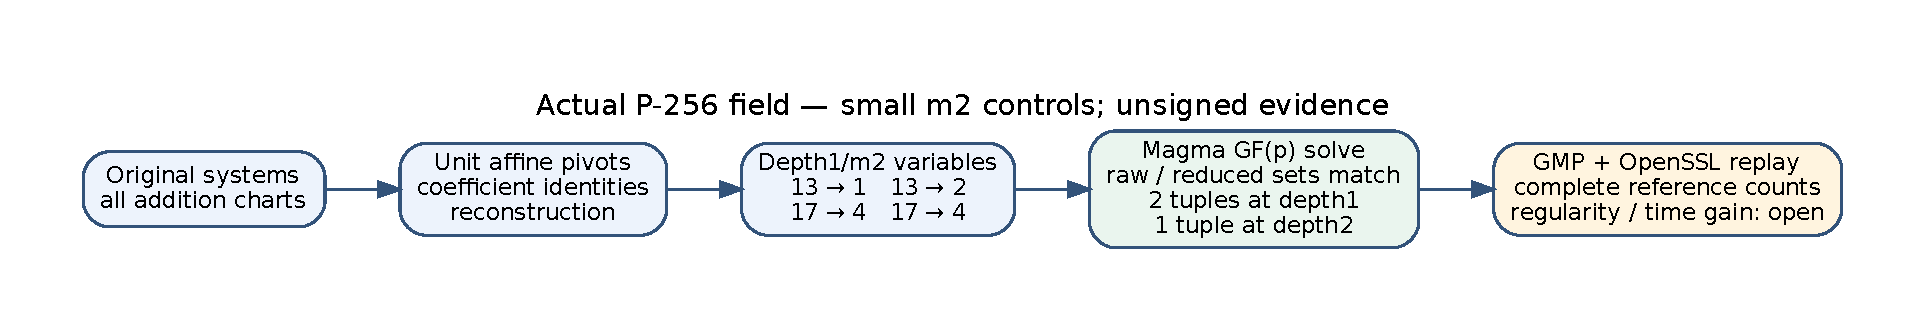
\includegraphics[width=\linewidth]{reduction.pdf}

\textbf{Controls.} Depth1/m2 uses \texttt{FB1hfa6130558c05}, one column/two
signed points, infinity target and two ordered relations. Depth2/m2 uses
\texttt{FB1hb6856918fe35}, two columns/four signed points, finite target
and one ordered relation. Both are planted controls. The field is not
replaced by a small prime. The original depth 4 nine-column fixture and
intended depth 8 m2--7 panel remain separate.

\textbf{Exact transformation.} For $a x+L=0$, constant $a\ne0$, substitute
$x=-L/a$ in every constraint and retain reconstruction expressions.
Native checks establish each pivot identity and
$f(x)-f(L)=(x-L)Q$ coefficient by coefficient, using a separate telescoping
construction. Only zero equations are dropped; no probabilistic relation
branch or exceptional chart is discarded. There are 72 native cases
(depths1/2/4, m2--7, four arms) and three corrupted-certificate controls
[pcc:unverified]. Linear elimination is standard, not a novelty claim.

\begin{center}
\begin{tabular}{llrrc}
\toprule
Control & Arm & Original vars & Residual vars & Raw/reduced GB degree\\\midrule
depth 1 & dense &13&1&2/2\\
depth 1 & tower &13&2&2/2\\
depth 1 & paired &17&4&2/2\\
depth 1 & oriented &17&4&2/2\\\midrule
depth 2 & dense &13&9&1/1\\
depth 2 & tower &15&11&1/1\\
depth 2 & paired &19&13&2/2\\
depth 2 & oriented &21&15&1/1\\\bottomrule
\end{tabular}
\end{center}
The table copies native metadata and CAS output on these controls only.
GB degree is the \textbf{affine output-basis degree}, not regularity or
maximum F4 matrix degree. Preprocessing did not lower this measured
degree. The depth 2 paired-to-oriented2-to-1 change concerns different
auxiliary covers with the same projected relation [pcc:unverified].

\textbf{Cover counts.} Raw and reduced dense/tower/oriented give 2 CAS
assignments at depth 1 and 1 at depth 2; paired gives 8 and 4. They project to
the same 2 or1 ordered tuples. Removing four auxiliary copies per relation
is not a fourfold runtime result. The infinity target has zero nonzero
projected coefficient rows; the finite target has one. Neither gives a
natural-yield or independent-rank result [pcc:unverified].

\newpage
\textbf{Actual execution.} Eight public requests: three rejected, five
admitted. Requests 004/006 run the raw four-arm cells,007/008 the reduced
cells,003 the field probe and first dense case. All 16 matched cells pass
complete counts and exact point replay [pcc:unverified]. Magma reports
version 2.30-1. Raw responses include all error flags and partial output.

\begin{center}
\begin{tabular}{rll}
\toprule
Request & Rejected behavior & Correction before later data\\\midrule
001 & thread control illegal; exit0 & remove public-unit thread control\\
002 & leading closer lost; stale ideal & join closer; SetQuitOnError\\
005 & Eltseq rejects tuple & explicit coordinate sequence\\\bottomrule
\end{tabular}
\end{center}
Two failed responses printed plausible markers after errors. Strict
whole-response admission rejected them. A marker/exit code alone is
insufficient. The public wrapper enables \texttt{SetIgnorePrompt(true)};
compatibility serialization preserves the frozen mathematical system.
Every failed source and response is retained [pcc:unverified].

\textbf{Provenance.} Requests 001--006 retain original input/request hashes
and source history, without separately copied immutable qualifiers.
Requests 007/008 add read-only qualifier/replayer copies and distinct
pre-call/post-call manifests. Later build metadata is labelled post-call.
The remote binary/image and host are not independently pinned. No signed
independent or execution-verified result is asserted.

Public units use one request at a time and a 25-second client cap; the
service advertises 1 GiB guest memory. Returned time/memory values are
retained but not used for a performance comparison. No EKS/L2 measurement,
2x gain, maximum F4 degree or structured regularity is established.

\textbf{Larger native-only scope.} At depth 4/m7, variable counts are
dense 83$\to$69, tower 104$\to$90, paired 118$\to$97 and oriented 139$\to$118.
Input degrees remain dense 9 and structured 3. Those cases have native
reconstruction checks but no CAS run here [pcc:unverified]. The intended
depth 8 m2--7 baseline and2x target remain open, with paid preprocessing,
conversion/replay and qualified backend accounting still required.

\textbf{Offline reproduction (no HTTP).}
\begin{verbatim}
research/p256_aux_smooth_20261114/continuation_20261116/\
run_checks.sh /tmp/aux-linear-001
\end{verbatim}
This rebuilds 72 native cases, compares coefficient certificate bytes,
replays all retained successful CAS results and rejects the recorded
errors and a malformed batch. No request is repeated. Source-linked
\texttt{REPORT.md}, protocols/amendments and all raw records accompany
this PDF; \texttt{evidence/cas-unit-matrix.json} is the complete matrix.

Main ledger synchronization retains its canonical prefix and appends
four unchanged unsigned claim bodies through \texttt{pcc.append\_entry}.
Lesson verification accepts 183 materialized entries. Another study's
record was not closed. Root release-lib cannot start locally (cargo
absent); no compiler-defect claim follows. CI/merge are pending publication
[pcc:unverified].

\textbf{Sources.}
\href{https://github.com/Magma-Maths/calculator/blob/main/README.md}{Calculator API},
wrapper app/magma\_cmd.py at 1e6267e22a19e75a6a3b6a3cc43bae3ce675e4a7;
\href{https://magma.maths.usyd.edu.au/magma/handbook/text/49}{environment options};
\href{https://magma.maths.usyd.edu.au/magma/handbook/text/1447}{linear elimination}.
Original PKM/source review remains in the parent report. KB unavailable;
no novelty inference. Key unsigned claims: PCC-20261116-e52985,6b5f12,2335a8.
\end{document}
